% Please name the set of problems ubgXX.tex, and the solutions lsgXX.tex, where XX is the number

\documentclass[11pt]{article}
\usepackage[german]{babel}
\usepackage{epsfig,graphicx}
\usepackage{amsmath}
%\usepackage{axodraw}
\usepackage{mathrsfs}
\usepackage{amsfonts}
\usepackage{slashed}
%\usepackage{txfonts, pxfonts}
\textheight 240mm
\textwidth 168mm
\topmargin -1.5cm
\oddsidemargin -4mm
\evensidemargin -4mm
\pagestyle{empty}
\parindent 0mm

% Commands for typesetting of the exercises/solutions: please do not edit them
\newenvironment{questions}{\begin{list}{\alph{enumi})}{\usecounter{enumi}\leftmargin6mm}}{\end{list}}
\newcounter{exercise}
\newcommand{\exercise}[1]{\vspace{0.5cm}\stepcounter{exercise} \noindent {\large {\bf \arabic{exercise}. #1}}\\[1mm] }
%\newcommand{\serie}[2]{\noindent{{\bf \mbox{Exercises for Kern- und Teilchenphysik II --- Prof.\,F.\,Canelli, Prof\,N.\,Serra--- \\Spring term 2015 - Exercise sheet 1}}}\\
\newcommand{\serie}[2]{ \bf{Exercises for Kern- und Teilchenphysik II} \\ Prof.\,F.\,Canelli, Prof\,N.\,Serra \\Spring term 2015 - Exercise sheet 1\\
\rule{\linewidth}{0.3mm} \\ \noindent{\it Issued: 27 February 2015\\ Due: 5 March 2015  \\Discussion: 5 March 2015  }\\[2mm]
 }
\newcommand{\solutions}[1]{\noindent{ {\bf \mbox{Einf\"uhrung in die Kern- und Teilchenphysik --- Prof.\,K.\,Kirch --- Serie #1}}}\\\rule{\linewidth}{0.5mm} \noindent{\it L\"osungen }\\[2mm]}


% The following commands are defined for your convenience, they work in both math and text mode
\def\epem{\ensuremath{\mathrm{e^+e^-}}}      % e+e-
\def\TeV{\ensuremath{\mathrm{\ Te\kern -0.1em V}}} % TeV in correct typesetting
\def\GeV{\ensuremath{\mathrm{\ Ge\kern -0.1em V}}} % GeV in correct typesetting
\def\MeV{\ensuremath{\mathrm{\ Me\kern -0.1em V}}} % MeV in correct typesetting
\def\keV{\ensuremath{\mathrm{\ ke\kern -0.1em V}}} % keV in correct typesetting
\def\eV{\ensuremath{\mathrm{\ e\kern -0.1em V}}} % eV in correct typesetting
\def\tev{\TeV{}} % same as above, for convenience
\def\gev{\GeV{}}
\def\mev{\MeV{}}
\def\kev{\keV{}}
\def\ev{\eV{}}
\def\Wp{\ensuremath{\mathrm {W^+}}} % W+ boson
\def\Wm{\ensuremath{\mathrm {W^-}}} % W- boson
\def\ra{\ensuremath{\rightarrow}} %  "GOES TO" arrow for reactions
\def\rts {\ensuremath{\sqrt{s}}} % square root of s
\newcommand{\La}{\ensuremath{\mathcal{L}}}  % Luminosity
\newcommand{\p}{\ensuremath{\partial}} %

\begin{document}
%%%%%%%%%%%%%%%%%%%%%%%%%%%%%%%%%%%%%%%%%%%%%%%%%%%%%%%%%%%%%
%   Uncomment the appropriate line:
%
%\serie{1}{}  % insert (1) problem set number and (2) deadline here
%\serie{1}{1./3./4. M\"{a}rz 2011}  % insert (1) problem set number and (2) deadline here
%
%\solutions{1}  % insert solutions number here
%
%%%%%%%%%%%%%%%%%%%%%%%%%%%%%%%%%%%%%%%%%%%%%%%%%%%%%%%%%%%%%



%\begin{minipage}
%\fontsize{14pt}{12pt}\fontsize{10pt}{12pt}
\large 
\textbf{
\centerline{Kern- und Teilchenphysik II}\\
\centerline{Spring Term 2015}\\
%\centerline{Prof.\,F.\,Canelli  Prof\,N.\,Serra}
\\
\Large \centerline{Exercise Sheet 2}
\\\\
}

\large
Lecturers: Prof.\,F.\,Canelli,  Prof.\,N.\,Serra\\
Assistants: Dr. M.\,Chrzaszcz, Dr. A.de Cosa

%Assistants: B. Casal Lara\~na, Dr. M. Doneg\`a, L. Tancredi, A. Torre\\
%\verb+https://moodle-app2.let.ethz.ch/course/view.php?id=1064+
%\end{minipage}
\normalsize


\exercise{Eigenspinors of the $S_{z}$ operator}

\begin{questions}

\item If the $z$ axis is orientated so that it points along the direction of motion, show that the canonical solution $u^{(1)}$ reduces to:
\begin{displaymath}
u^{(1)} = \begin{pmatrix}
  \sqrt{(E + mc^{2})/c} \\
  0 \\
  \sqrt{(E - mc^{2})/c} \\
  0 \\
\end{pmatrix}
\end{displaymath}

\item Construct the equivalent expressions for $u^{(2)}$, $v^{(1)}$ and $v^{(2)}$
\item Show that they are all eigenspinors of $S_{z}$, and find their eigenvalues
\end{questions}

\exercise{Electron-muon scattering}

%The amplitude for electron-positron scattering is given by:
Let's consider electron-positron scattering happens by the two diagrams shown below:
%\begin{displaymath}
%\mathcal{M} = -\frac{g^{2}_{e}}{(p_{1}-p_{3})^2}[\bar{u}(3)\gamma^{\mu}u(1))] [\bar{\nu}(2)\gamma^{\mu}\nu(4))] + \frac{g^{2}_{e}}{(p_{1}+p_{2})^2}[\bar{\nu}(3)\gamma^{\nu}\nu(4))] [\bar{u}(2)\gamma^{\nu}u(1))] 
%\end{displaymath}
\center{
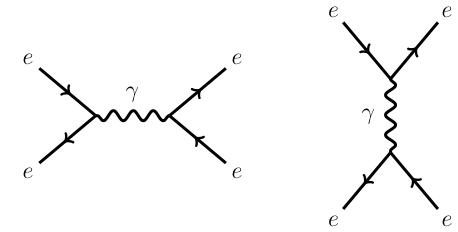
\includegraphics[width=0.4\textwidth]{eetoee1.png}
}

\begin{questions}
\item Usin Feyman rules please write down the amplitude for the sum od the two processes.
\item Evaluate the amplitude for electron-positron scattering in the CM system, assuming the $e^-$ and $e^+$ approach each other along the $z$ axis, repel, and return along the $z$ axis.  Assume the initial and final particles all have helicity +1. [Hint: Use the spinors you calculated in the previous question]

\end{questions}

\exercise{Casimir's trick}

Casimir's trick states that: 

\begin{displaymath}
\sum_{\text{all spins}} [\bar{u}(a)\Gamma_{1}u(b)][\bar{u}(a)\Gamma_{2}u(b)]^{*} = \text{Tr}[\Gamma_{1}(\slashed{p_{b}}+m_{b}c)\overline{\Gamma}_{2}(\slashed{p_{a}}+m_{a}c)]
\end{displaymath}

\begin{questions}
\item Find the analogue expression for antiparticles:
\begin{displaymath}
\sum_{\text{all spins}} [\bar{v}(a)\Gamma_{1}v(b)][\bar{v}(a)\Gamma_{2}v(b)]^{*} 
\end{displaymath}

\end{questions}

\end{document}
